\documentclass[handout]{beamer}
%\usetheme{Boadilla}
%\usetheme{Szeged}
%\usetheme{Singapore}
\usetheme{Frankfurt}
\usecolortheme{dove}
\newenvironment{alltt}{\ttfamily}{\par}
\usepackage{amsmath,amssymb,amsfonts,amsthm, multicol, subfigure, color}
\usepackage{bm}
\usepackage{graphicx}
\usepackage{hyperref}
\definecolor{dodgerblue}{rgb}{.118, .575, 1}
\def\independenT#1#2{\mathrel{\rlap{$#1#2$}\mkern2mu{#1#2}}}
\newcommand\independent{\protect\mathpalette{\protect\independenT}{\perp}}
\newcommand\indep{\protect\mathpalette{\protect\independenT}{\perp}}
\usepackage{tikz}
\usetikzlibrary{arrows,shapes.arrows,positioning,shapes}
\newcommand{\red}{\textcolor{red}}
\newcommand{\blue}[1]{\textcolor{blue}{#1}}
\newcommand{\black}[1]{\textcolor{black}{#1}}
\newcommand{\purple}[1]{\textcolor{purple}{#1}}
\newcommand{\green}[1]{\textcolor{olive}{#1}}
\newcommand{\white}[1]{\textcolor{white}{#1}}
\newcommand{\bblue}[1]{\textbf{\textcolor{blue}{#1}}}
\newcommand{\bgreen}[1]{\textbf{\color{olive}{#1}}}
\renewcommand{\d}{\text{d}}
\newcommand{\E}{\text{E}}
\newcommand{\V}{\text{V}}
\renewcommand{\P}{\text{P}}

\title{\blue{Precept 4 - More GLMs: \\ Models of Binary Outcomes}}
\subtitle{\green{Soc 504: Advanced Social Statistics}}
\author{Ian Lundberg\footnote{These slides owe an enormous debt to generations of TFs in Gov 2001 at Harvard. Many slides are directly adapted from those by Brandon Stewart and Stephen Pettigrew.}}
\institute[Princeton]{Princeton University}
\date{March 2, 2018}

\begin{document}

\frame{\titlepage}

\begin{frame}
\frametitle{Outline}
\tableofcontents
\end{frame}

\begin{frame}
\frametitle{Replication Paper}
\huge \blue{Anything to discuss?}
\end{frame}

\begin{frame}{To discuss from a card}
\large I would love it if the preceptors would be really honest about priorities in the homework. How should we prioritize the different elements each week? Especially weeks we're drowning other work? (1) Pset, (2) Replication? Reading?
\end{frame}

\begin{frame}{A framework for doing research}
\begin{center}\begin{tikzpicture}[x = .5\textwidth, y = .5\textheight]
\node[align=left, text width = \textwidth] at (0,0) {
\begin{enumerate}
\item Define a quantity of interest $\tau$
\item Specify a model and maximize the likelihood to estimate $\hat\theta$
\item Calculate the MLE for your quantity of interest: $\hat\tau = h(\hat\theta)$
\item Simulate estimation uncertainty. Do the following thousands of times:
\begin{enumerate}
\item Draw $\tilde\theta$ from its theoretical sampling distribution
\item Calculate your quantity of interest $\tilde\tau = h\left(\tilde\theta\right)$
\end{enumerate}
\item Report your point estimate from (3) and a 95\% confidence interval from (4) in an informative graph.
\end{enumerate}
};
\onslide<2-2>{
\node[blue] (soc) at (0.5, 0.7) {This is social science!};
\draw[->, blue, thick] (soc) to[bend left = 20] (0.07, 0.45);
\node[olive, align = center] (auto) at (-.8,0.7) {This should\\feel automatic};
\draw[->, olive, thick] (auto) to[bend right = 50] (-1, 0.2);
\draw[->, olive, thick] (auto) to[bend right = 50] (-1, 0.1);
\node[purple] (comm) at (0,-.7) {Communication matters!};
\draw[->, purple, thick] (0.4,-.7) to[bend right = 80] (0.4, -.5);
}
\end{tikzpicture}\end{center}
\end{frame}

\section{Define a quantity of interest}

\begin{frame}
\begin{center}

\includegraphics[scale=.5]{figs/desmond_evicted_2016_cover.jpeg}
\end{center}
\end{frame}

\begin{frame}
We will use data from the Fragile Families and Child Wellbeing Study to study the probability of eviction for children born in large American cities. \vskip .5cm


\includegraphics[width=.8\textwidth]{figs/ff_logo.jpg}

\end{frame}

\begin{frame}[fragile]{Fragile Families data}
\texttt{ffEviction.dta} contains these data. \vskip .5cm
\small
\texttt{evicted}: was this child evicted in a given year? \vskip .2cm
\texttt{income}: family income / poverty line at age 1 \vskip .2cm
\texttt{married}: were the parents married at the birth? \vskip .2cm
\texttt{race}: mother's race/ethnicity \vskip .2cm
\texttt{m1natwt}: sample weight
\end{frame}

\begin{frame}[fragile]
\frametitle{Fragile Families data}
\small
\begin{semiverbatim}
  idnum evicted income married     race  m1natwt
1  0001   FALSE    1.5   FALSE Hispanic  5.06258
2  0003   FALSE    2.7   FALSE    White 12.91446
3  0004   FALSE    1.0   FALSE Hispanic 36.08243
4  0006   FALSE    0.2   FALSE    Black 79.70869
5  0007   FALSE    1.3   FALSE Hispanic 31.66235
6  0008   FALSE    0.5   FALSE    Black 65.91409
\end{semiverbatim}
\end{frame}

\begin{frame}{A framework for doing research}
\begin{center}\begin{tikzpicture}[x = .5\textwidth, y = .5\textheight]
\node[align=left, text width = \textwidth] at (0,0) {
\begin{enumerate}
\item Define a quantity of interest $\tau$
\item Specify a model and maximize the likelihood to estimate $\hat\theta$
\item Calculate the MLE for your quantity of interest: $\hat\tau = h(\hat\theta)$
\item Simulate estimation uncertainty. Do the following thousands of times:
\begin{enumerate}
\item Draw $\tilde\theta$ from its theoretical sampling distribution
\item Calculate your quantity of interest $\tilde\tau = h\left(\tilde\theta\right)$
\end{enumerate}
\item Report your point estimate from (3) and a 95\% confidence interval from (4) in an informative graph.
\end{enumerate}
};
\node[blue] (soc) at (0.5, 0.7) {This is social science!};
\draw[->, blue, thick] (soc) to[bend left = 20] (0.07, 0.45);
\node[olive, align = center] (auto) at (-.8,0.7) {This should\\feel automatic};
\draw[->, olive, thick] (auto) to[bend right = 50] (-1, 0.2);
\draw[->, olive, thick] (auto) to[bend right = 50] (-1, 0.1);
\node[purple] (comm) at (0,-.7) {Communication matters!};
\draw[->, purple, thick] (0.4,-.7) to[bend right = 80] (0.4, -.5);
\end{tikzpicture}\end{center}
\end{frame}

\begin{frame}{1. Define a quantity of interest $\tau$}
\begin{footnotesize}\blue{Note:} I use the general notation (i.e. $\tau$, $\theta$) in the slide titles and the specific application notation in the slide text. $\tau$ represents a generic quantity of interest; $\pi$ represents the particular quantity of interest in this example. Fitting a particular example into a general framework is a key goal of the course!\end{footnotesize} \vskip .5cm \pause
$\pi$ = probability of eviction in a calendar year for
\begin{itemize}
\item a white child
\item born in 1998-2000
\item to married parents
\item living at the poverty line
\item in an American city with population over 200,000
\end{itemize}
\end{frame}

\begin{frame}
\bblue{Research question:} What is the probability of eviction in a calendar year for a white child born in 1998-2000 to married parents living at the poverty line in an American city with population over 200,000? \vskip .2cm \pause
\bgreen{A simple strategy:}
\begin{itemize}
\item There are 3,442 observations in the data.
\item There are 7 observations meeting this description.
\item One could report the proportion of these who are evicted.
\end{itemize} \pause
\bgreen{Think, pair, share}:
\begin{itemize}
\item \bblue{Q:} What are the advantages of this model-free approach?
\begin{itemize}
\onslide<4->{\item \bgreen{A:} It is unbiased, simple to understand, and requires minimal assumptions!}
\end{itemize}
\item \bblue{Q:} Why might one prefer a parametric model?
\begin{itemize}
\onslide<5->{\item \bgreen{A:} The model-free approach is very noisy. There are only 7 observations! We gain efficiency by assuming a parametric model in order to \bblue{share information} from other observations.}
\end{itemize}
\end{itemize}
\end{frame}

\section{Fit a model}

\begin{frame}{A framework for doing research}
\begin{center}\begin{tikzpicture}[x = .5\textwidth, y = .5\textheight]
\node[align=left, text width = \textwidth] at (0,0) {
\begin{enumerate}
\item Define a quantity of interest $\tau$
\item Specify a model and maximize the likelihood to estimate $\hat\theta$
\item Calculate the MLE for your quantity of interest: $\hat\tau = h(\hat\theta)$
\item Simulate estimation uncertainty. Do the following thousands of times:
\begin{enumerate}
\item Draw $\tilde\theta$ from its theoretical sampling distribution
\item Calculate your quantity of interest $\tilde\tau = h\left(\tilde\theta\right)$
\end{enumerate}
\item Report your point estimate from (3) and a 95\% confidence interval from (4) in an informative graph.
\end{enumerate}
};
\node[blue] (soc) at (0.5, 0.7) {This is social science!};
\draw[->, blue, thick] (soc) to[bend left = 20] (0.07, 0.45);
\node[olive, align = center] (auto) at (-.8,0.7) {This should\\feel automatic};
\draw[->, olive, thick] (auto) to[bend right = 50] (-1, 0.2);
\draw[->, olive, thick] (auto) to[bend right = 50] (-1, 0.1);
\node[purple] (comm) at (0,-.7) {Communication matters!};
\draw[->, purple, thick] (0.4,-.7) to[bend right = 80] (0.4, -.5);
\end{tikzpicture}\end{center}
\end{frame}

\begin{frame}{Generalized Linear Models: Three elements}
$$\overbrace{\vec{X_i}\vec\beta = \eta_i}^\text{\bgreen{Linear predictor}}$$
$$\overbrace{\eta_i = g(\mu_i)}^\text{\bgreen{Link function $g$}}$$
$$\overbrace{Y_i \sim f_Y(\mu_i,\gamma)}^\text{\bgreen{Stochastic component}}$$
\end{frame}

\begin{frame}
Specify a distribution for $Y$ \pause \\ 
\begin{center}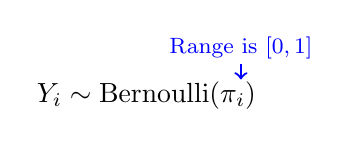
\begin{tikzpicture}
	\node at (0,0) {$Y_i \sim \mathrm{Bernoulli}(\pi_i)$};
	\node[blue, font = \footnotesize] at (1.2,.6) {Range is $[0,1]$};
	\draw[->, blue, thick] (1.2,.4) -- (1.2,.2);
\end{tikzpicture}\end{center}

Specify a linear predictor: \pause \\ 
\begin{center}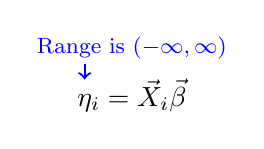
\begin{tikzpicture}
	\node at (0,0) {$\eta_i = \vec{X}_i\vec\beta$};
	\node[blue, font = \footnotesize] at (0,.6) {Range is $(-\infty,\infty)$};
	\draw[->, blue, thick] (-.6,.4) -- (-.6,.2);
\end{tikzpicture}\end{center}

Specify a link function $\eta_i = g(\pi_i)$ \pause \vskip .2cm
Complementary Log-log (cloglog):
$$\eta_i = g(\pi_i) = \green{\underbrace{\log(\blue{\overbrace{-\log(1-\pi_i)}^\text{Range is $(0,\infty)$}})}_\text{Range is $(-\infty,\infty)$}}$$
\end{frame}

\begin{frame}
Our complementary log-log \blue{link function} is 
$$\vec{X}_i\vec\beta = \eta_i = g(\pi_i) = \green{\underbrace{\log(\blue{\overbrace{-\log(1-\pi_i)}^\text{Range is $(0,\infty)$}})}_\text{Range is $(-\infty,\infty)$}}$$ \pause
We can solve for $\pi_i$ to get the \blue{inverse link function} \pause
$$\begin{aligned}
\vec{X}_i\vec\beta &= \overbrace{\log(-\log(1-\pi_i))}^\text{\green{Link function $g$}} \\ \pause
\exp(\vec{X}_i\vec\beta) &= -\log(1-\pi_i) \\ \pause
\exp(-\exp(\vec{X}_i\vec\beta)) &= 1 - \pi_i \\ \pause
\underbrace{1 - \exp(-\exp(\vec{X}_i\vec\beta))}_\text{\green{Inverse link function $g^{-1}$}} &= \pi_i
\end{aligned}$$
\end{frame}

\begin{frame}
There are \blue{many link functions} for binary outcomes: \\
\begin{itemize}
\item \green{Complementary log-log:} $\eta_i = g(\pi_i) = \log(-\log(1-\pi_i))$
\item \green{Probit:} $\eta_i = g(\pi_i) = \Phi^{-1}(\pi_i)$
\item \green{Logit:} $\eta_i = g(\pi_i) = \log\left(\frac{\pi_i}{1- \pi_i}\right)$
%\item \green{Scobit:} $\pi_i = (1+e^{-x_i \beta})^{-\alpha}$ commented out because this is confusing
\end{itemize}
\end{frame}

\begin{frame}
\frametitle{Log-likelihood of the c-loglog}
\pause
\begin{scriptsize}
$$\begin{aligned}
\ell(\vec\beta \mid \vec{Y}) &= \log(L(\vec\beta \mid \vec{Y})) \\ \pause
&= \log(p(\vec{Y}\mid \vec\beta,\mathbf{X})) \\\pause
&= \log\left(\prod_{i=1}^n p(Y_i\mid \vec\beta, \vec{X}_i)\right) \qquad \pause \blue{\leftarrow \text{ assumes independence conditional on }\mathbf{X}} \\\pause
&= \log\left(\prod_{i=1}^n [1 - \exp(-\exp(\vec{X}_i\vec\beta))]^{Y_i}[\exp(-\exp(\vec{X}_i\vec\beta))]^{(1-Y_i)}\right) \\\pause
&= \sum_{i=1}^n \left( Y_i\log(1 - \exp(-\exp(\vec{X}_i\vec\beta))) + (1-Y_i)\log[\exp(-\exp(\vec{X}_i\vec\beta))]\right) \\\pause
&= \sum_{i=1}^n \left( Y_i\log(1 - \exp(-\exp(\vec{X}_i\vec\beta))) - (1-Y_i)\exp(\vec{X}_i\vec\beta)\right) \\
\end{aligned}$$
\end{scriptsize}
\end{frame}

\begin{frame}[fragile]
\frametitle{Coding our log likelihood function}
$$\sum_{i=1}^n \left( Y_i\log(1 - \exp(-\exp(\vec{X}_i\vec\beta))) - (1-Y_i)\exp(\vec{X}_i\vec\beta)\right)$$
\pause

\begin{semiverbatim}
cloglog.loglik <- function(par, X, y) \{
\end{semiverbatim}
\pause
\begin{semiverbatim}
     beta <- par
\end{semiverbatim}
\pause
\begin{semiverbatim}
     log.lik <- sum(y * log(1 - exp(-exp(X \%*\% beta))) -
                   (1 - y) * exp(X \%*\% beta))
\end{semiverbatim}
\pause
\begin{semiverbatim}
  return(log.lik)
\}
\end{semiverbatim}
\end{frame}

\begin{frame}[fragile]
\frametitle{Finding the MLE}
\pause
\begin{semiverbatim}
X <- model.matrix(~married + race + income,
                  data = d)
\end{semiverbatim}
\pause
\begin{semiverbatim}
opt <- optim(par = rep(0, ncol(X)),
\end{semiverbatim}
\pause
\begin{semiverbatim}
             fn = cloglog.loglik,
\end{semiverbatim}
\pause
\begin{semiverbatim}
             X = X,
             y = d$ev,
\end{semiverbatim}
\pause
\begin{semiverbatim}
             control = list(fnscale = -1),
\end{semiverbatim}
\pause
\begin{semiverbatim}
             hessian = T,
\end{semiverbatim}
\pause
\begin{semiverbatim}
             method = "BFGS")
\end{semiverbatim}
\pause
{\bf Point estimate of the MLE}:
\begin{semiverbatim}
opt$par
[1] -2.9980367 -1.0960323 -0.1799426  0.2055103  0.5671903 -0.1779315
\end{semiverbatim}
\end{frame}

\begin{frame}[fragile]
\frametitle{Standard errors of the MLE}
\pause
Recall that the standard errors are defined as the diagonal of:\\

$$\sqrt{-\bigg[ \frac{\partial^2 \ell}{\partial\beta^2}\bigg] ^{-1}}$$
\pause
\begin{multicols}{2}
\raggedleft
where $\frac{\partial^2 \ell}{\partial\beta^2}$ is the\\ \pause
\columnbreak
\raggedright
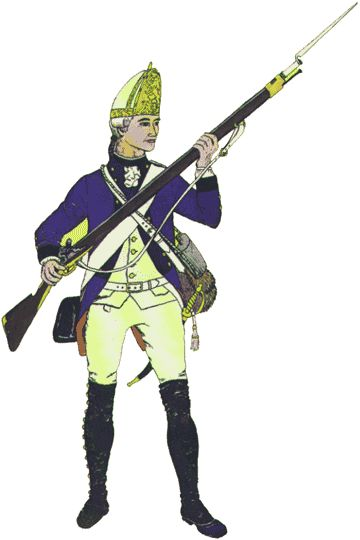
\includegraphics[scale=.2]{figs/hessian}\footnote{Credit to Stephen Pettigrew for including this figure in slides.\vskip .2cm}
\end{multicols}
\end{frame}


\begin{frame}[fragile]
\frametitle{Standard errors of the MLE}
\pause
\bblue{Variance-covariance matrix}:
\begin{semiverbatim}
-solve(opt$hessian)
\end{semiverbatim}
\begin{scriptsize}\begin{tabular}{rrrrrrr}
  \hline
 & (Intercept) & married & raceBlack & raceHispanic & raceOther & income \\ 
  \hline
(Intercept) & 0.08 & -0.01 & -0.06 & -0.06 & -0.05 & -0.01 \\ 
  married & -0.01 & 0.14 & 0.01 & 0.01 & -0.00 & -0.01 \\ 
  raceBlack & -0.06 & 0.01 & 0.08 & 0.06 & 0.05 & 0.01 \\ 
  raceHispanic & -0.06 & 0.01 & 0.06 & 0.08 & 0.05 & 0.01 \\ 
  raceOther & -0.05 & -0.00 & 0.05 & 0.05 & 0.22 & 0.00 \\ 
  income & -0.01 & -0.01 & 0.01 & 0.01 & 0.00 & 0.01 \\ 
   \hline
\end{tabular}\end{scriptsize}
\pause \vskip .2cm
\bblue{Standard errors}: Square root of the diagonal
\begin{scriptsize}
\begin{semiverbatim}
sqrt(diag(-solve(opt$hessian)))

 (Intercept)      married    raceBlack raceHispanic    raceOther       income 
       0.276        0.370        0.281        0.280        0.466        0.088 
\end{semiverbatim}
\end{scriptsize}
\end{frame}

\begin{frame}{Interpreting c-loglog coefficients}
\pause
Here's a nicely formatted table with your regression results from our model:\\

% latex table generated in R 3.4.3 by xtable 1.8-2 package
% Thu Mar  1 22:12:09 2018
\begin{table}[ht]
\centering
\begin{tabular}{lrr}
  \hline
Variable & Coefficient & SE \\ 
  \hline
Intercept & -3.00 & 0.28 \\ 
  Married & -1.10 & 0.37 \\ 
  Black & -0.18 & 0.28 \\ 
  Hispanic & 0.21 & 0.28 \\ 
  Other & 0.57 & 0.47 \\ 
  Income / poverty line & -0.18 & 0.09 \\ 
   \hline
\end{tabular}
\end{table}

\pause
\begin{center}
But what does this table tell us?
\end{center}
\end{frame}

\begin{frame}
\frametitle{Interpreting c-loglog results}
What does it mean for the coefficient for married to be -1.10?\\
\pause
\bigskip
All else constant, children of married parents have -1.10 points lower log rate of eviction. \\
\pause
\bigskip
Was that the kind of question that inspired you to become a social scientist?
\pause
What are log rates? \pause
Nobody thinks in terms of log odds, or probit coefficients, or exponential rates.
\end{frame}

\begin{frame}
If there's one thing you take away from this class, it should be this:\\
\pause
\bigskip
\centering \textcolor{blue}{\Large When you present results, {\bf always} present your findings in terms of something that has substantive meaning to the reader.}\\

\bigskip
\pause 
\raggedright For binary outcome models that often means turning your results into predicted probabilities, which is what we'll do now.

\bigskip
\pause
If there's a second thing you should take away, it's this:\\
\pause
\bigskip
\centering \textcolor{blue}{\Large Always account for all types of uncertainty when you present your results}\\

\bigskip
\pause
\raggedright We'll spend the rest of today looking at how to do that.
\end{frame}

\section{Estimate your quantity of interest}

\begin{frame}{A framework for doing research}
\begin{center}\begin{tikzpicture}[x = .5\textwidth, y = .5\textheight]
\node[align=left, text width = \textwidth] at (0,0) {
\begin{enumerate}
\item Define a quantity of interest $\tau$
\item Specify a model and maximize the likelihood to estimate $\hat\theta$
\item Calculate the MLE for your quantity of interest: $\hat\tau = h(\hat\theta)$
\item Simulate estimation uncertainty. Do the following thousands of times:
\begin{enumerate}
\item Draw $\tilde\theta$ from its theoretical sampling distribution
\item Calculate your quantity of interest $\tilde\tau = h\left(\tilde\theta\right)$
\end{enumerate}
\item Report your point estimate from (3) and a 95\% confidence interval from (4) in an informative graph.
\end{enumerate}
};
\node[blue] (soc) at (0.5, 0.7) {This is social science!};
\draw[->, blue, thick] (soc) to[bend left = 20] (0.07, 0.45);
\node[olive, align = center] (auto) at (-.8,0.7) {This should\\feel automatic};
\draw[->, olive, thick] (auto) to[bend right = 50] (-1, 0.2);
\draw[->, olive, thick] (auto) to[bend right = 50] (-1, 0.1);
\node[purple] (comm) at (0,-.7) {Communication matters!};
\draw[->, purple, thick] (0.4,-.7) to[bend right = 80] (0.4, -.5);
\end{tikzpicture}\end{center}
\end{frame}

\begin{frame}{3. Calculate the MLE for our quantity of interest $\tau = h(\theta)$}

Our complementary log-log \blue{link function} is 
$$g(\pi_i) = \green{\underbrace{\log(\blue{\overbrace{-\log(1-\pi_i)}^\text{Range is $(0,\infty)$}})}_\text{Range is $(-\infty,\infty)$}} \qquad g(\pi_i) = X_i\beta$$ \pause
To go from a covariate set $X_i$ to a predicted probability, we use the \blue{inverse link function} \pause
$$\begin{aligned}
\vec{X}_i\vec\beta &= \overbrace{\log(-\log(1-\pi_i))}^\text{\green{Link function $g$}} \\
\underbrace{1 - \exp(-\exp(\vec{X}_i\vec\beta))}_\text{\green{Inverse link function $g^{-1}(X_i\beta)$}} &= \pi_i
\end{aligned}$$

The predicted probability of eviction for a child with covariates $\vec{x}$ is
$$\pi = h(\vec{x},\vec\beta) = g^{-1}(\vec{x}\vec\beta) = 1 - \exp(-\exp(\vec{x}\vec\beta))$$

\end{frame}

\begin{frame}[fragile]{Calculate the MLE for our quantity of interest $\tau = h(\theta)$}
The predicted probability of eviction for a child with covariates $\vec{x}$ is
$$\pi = h\left(\vec{x},\vec\beta\right) = g^{-1}\left(\vec{x}\vec\beta\right) = 1 - \exp\left(-\exp\left(\vec{x}\vec\beta\right)\right)$$
$$\hat\pi_\text{MLE} = h\left(\vec{x},\hat{\vec\beta}_\text{MLE}\right) = g^{-1}\left(\vec{x}\hat{\vec\beta}_\text{MLE}\right) = 1 - \exp\left(-\exp\left(\vec{x}\hat{\vec\beta}_\text{MLE}\right)\right)$$
\bblue{In code:}
\begin{footnotesize}
\begin{semiverbatim}
get.pred.prob <- function(setX, beta) \{
  ## Calculate the linear predictor
  eta <- setX %*% beta
  ## Transform by the inverse link function
  prob <- 1 - exp(-exp(eta))
  return(prob)
\}
\end{semiverbatim}
\end{footnotesize}
\end{frame}

\begin{frame}[fragile]
\frametitle{Calculate the MLE for our quantity of interest $\tau = h(\theta)$}
\pause
Now we need to choose some values of the covariates that we want predictions about.\\
\pause
\bigskip
Let's make predictions for one white child born to married parents with family income at the poverty line
Recall that our predictors (in order) are:
\begin{tiny}
\begin{semiverbatim}
> colnames(X)
[1] "(Intercept)"        "married"            "cm1ethraceBlack"    "cm1ethraceHispanic"
[5] "cm1ethraceOther"    "income" 
\end{semiverbatim}
\end{tiny}
We can \blue{set the values of $X$} as:
\pause
\begin{semiverbatim}
setX <- c(1, 1, 0, 0, 0, 1)
pi_hat <- get.pred.prob(setX = setX, beta = opt$par)
\end{semiverbatim}
We estimate that the probability of eviction is \blue{$\hat\pi = 0.014$.}
\end{frame}

\begin{frame}
\centering \huge But how \blue{certain} are we of that estimate?
\end{frame}

\section{Simulate uncertainty}

\begin{frame}{A framework for doing research}
\begin{center}\begin{tikzpicture}[x = .5\textwidth, y = .5\textheight]
\node[align=left, text width = \textwidth] at (0,0) {
\begin{enumerate}
\item Define a quantity of interest $\tau$
\item Specify a model and maximize the likelihood to estimate $\hat\theta$
\item Calculate the MLE for your quantity of interest: $\hat\tau = h(\hat\theta)$
\item Simulate estimation uncertainty. Do the following thousands of times:
\begin{enumerate}
\item Draw $\tilde\theta$ from its theoretical sampling distribution
\item Calculate your quantity of interest $\tilde\tau = h\left(\tilde\theta\right)$
\end{enumerate}
\item Report your point estimate from (3) and a 95\% confidence interval from (4) in an informative graph.
\end{enumerate}
};
\node[blue] (soc) at (0.5, 0.7) {This is social science!};
\draw[->, blue, thick] (soc) to[bend left = 20] (0.07, 0.45);
\node[olive, align = center] (auto) at (-.8,0.7) {This should\\feel automatic};
\draw[->, olive, thick] (auto) to[bend right = 50] (-1, 0.2);
\draw[->, olive, thick] (auto) to[bend right = 50] (-1, 0.1);
\node[purple] (comm) at (0,-.7) {Communication matters!};
\draw[->, purple, thick] (0.4,-.7) to[bend right = 80] (0.4, -.5);
\end{tikzpicture}\end{center}
\end{frame}

\begin{frame}{4. Simulate estimation uncertainty}

We have \blue{estimation} and \green{fundamental} uncertainty about $Y$. \vskip .2cm
In most models, we have to account for both types of uncertainty. \vskip .5cm
In this case, our quantity of interest $\pi = E(Y)$. \vskip .2cm
We are uncertain about $\pi$ only because we are uncertain about $\beta$ (\blue{estimation uncertainty}). \vskip .2cm
\begin{center}\Large Let's capture that uncertainty!\end{center}

\end{frame}

\begin{frame}[fragile]{4. Simulate estimation uncertainty}
$$\tilde\beta \sim \text{Normal}\left(\hat\beta,\hat\V(\hat\beta)\right)$$
$$\tilde\pi = h(x,\tilde\beta)$$
Take one draw of $\tilde\pi$.
\begin{footnotesize}\begin{semiverbatim}
draw.sim.prob <- function(setX, beta\_hat, vcov\_beta\_hat) \{
  beta\_tilde <- t(rmvnorm(n = 1,
                          mean = beta\_hat,
                          sigma = vcov\_beta\_hat))
  prob\_tilde <- get.pred.prob(setX = setX, beta = beta\_tilde)
  return(prob_tilde)
\}
\end{semiverbatim}\end{footnotesize}
\end{frame}

\begin{frame}[fragile]{4. Simulate estimation uncertainty}
$$\tilde\beta \sim \text{Normal}\left(\hat\beta,\hat\V(\hat\beta)\right)$$
$$\tilde\pi = h(x,\tilde\beta)$$
Take many draws of $\tilde\pi$.
\begin{footnotesize}\begin{semiverbatim}
beta\_hat <- opt$par
vcov\_beta\_hat <- -solve(opt$hessian)
set.seed(08544)
draws <- replicate(20000, draw.sim.prob(setX = setX,
                                        beta\_hat = beta\_hat,
                                        vcov\_beta\_hat = vcov\_beta\_hat))
\end{semiverbatim}\end{footnotesize}
\end{frame}

\section{Report results}

\begin{frame}{A framework for doing research}
\begin{center}\begin{tikzpicture}[x = .5\textwidth, y = .5\textheight]
\node[align=left, text width = \textwidth] at (0,0) {
\begin{enumerate}
\item Define a quantity of interest $\tau$
\item Specify a model and maximize the likelihood to estimate $\hat\theta$
\item Calculate the MLE for your quantity of interest: $\hat\tau = h(\hat\theta)$
\item Simulate estimation uncertainty. Do the following thousands of times:
\begin{enumerate}
\item Draw $\tilde\theta$ from its theoretical sampling distribution
\item Calculate your quantity of interest $\tilde\tau = h\left(\tilde\theta\right)$
\end{enumerate}
\item Report your point estimate from (3) and a 95\% confidence interval from (4) in an informative graph.
\end{enumerate}
};
\node[blue] (soc) at (0.5, 0.7) {This is social science!};
\draw[->, blue, thick] (soc) to[bend left = 20] (0.07, 0.45);
\node[olive, align = center] (auto) at (-.8,0.7) {This should\\feel automatic};
\draw[->, olive, thick] (auto) to[bend right = 50] (-1, 0.2);
\draw[->, olive, thick] (auto) to[bend right = 50] (-1, 0.1);
\node[purple] (comm) at (0,-.7) {Communication matters!};
\draw[->, purple, thick] (0.4,-.7) to[bend right = 80] (0.4, -.5);
\end{tikzpicture}\end{center}
\end{frame}

\begin{frame}{5. Report results}
We recommend reporting
\begin{itemize}
\item your point estimate $\hat\tau$ \onslide<2->{(the MLE by the invariance property)}
\item a 95\% quantile-based confidence interval
\end{itemize}
\onslide<3->{
\begin{center}
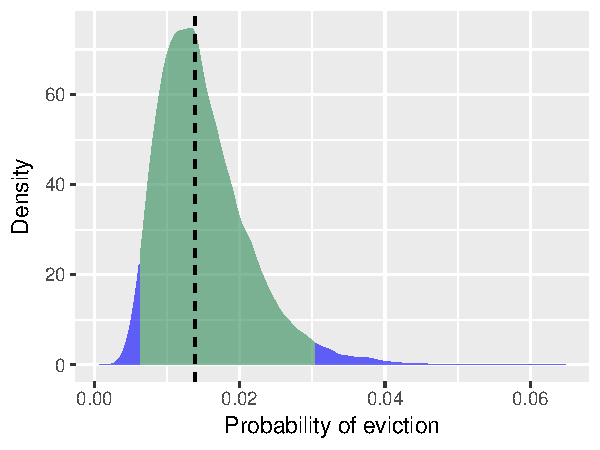
\includegraphics[width=.6\textwidth]{figs/pred_prob}
\end{center}
}
\end{frame}

\begin{frame}{A framework for doing research}
\begin{center}\begin{tikzpicture}[x = .5\textwidth, y = .5\textheight]
\node[align=left, text width = \textwidth] at (0,0) {
\begin{enumerate}
\item Define a quantity of interest $\tau$
\item Specify a model and maximize the likelihood to estimate $\hat\theta$
\item Calculate the MLE for your quantity of interest: $\hat\tau = h(\hat\theta)$
\item Simulate estimation uncertainty. Do the following thousands of times:
\begin{enumerate}
\item Draw $\tilde\theta$ from its theoretical sampling distribution
\item Calculate your quantity of interest $\tilde\tau = h\left(\tilde\theta\right)$
\end{enumerate}
\item Report your point estimate from (3) and a 95\% confidence interval from (4) in an informative graph.
\end{enumerate}
};
\node[blue] (soc) at (0.5, 0.7) {This is social science!};
\draw[->, blue, thick] (soc) to[bend left = 20] (0.07, 0.45);
\node[olive, align = center] (auto) at (-.8,0.7) {This should\\feel automatic};
\draw[->, olive, thick] (auto) to[bend right = 50] (-1, 0.2);
\draw[->, olive, thick] (auto) to[bend right = 50] (-1, 0.1);
\node[purple] (comm) at (0,-.7) {Communication matters!};
\draw[->, purple, thick] (0.4,-.7) to[bend right = 80] (0.4, -.5);
\end{tikzpicture}\end{center}
\end{frame}

\section{Practice 1}

\begin{frame}
\Huge\centering \blue{More practice.}
\end{frame}

\begin{frame}
\frametitle{Different quantity of interest}
\pause
How does the probability of eviction vary by family income? \\
We will set $\vec{x}$ to represent a white child born to married parents and will vary the family income between \blue{twice the poverty line} and \blue{half the poverty line}.
$$\begin{aligned}
\pi_\text{Twice} &= \P\left(Y\mid \vec{x}_\text{Twice poverty line}\right) \\
\pi_\text{Half} &= \P\left(Y\mid \vec{x}_\text{Half poverty line}\right) \\
\end{aligned}$$
\pause
$$\begin{aligned}
\tau &= \pi_\text{Twice} - \pi_\text{Half}
\end{aligned}$$
\bigskip
The model is the same. We just changed the quantity of interest.
\end{frame}

\begin{frame}{\blue{Pause:} Under what conditions is $\tau$ causal?}
$\tau$ represents the difference in the predicted probability of eviction between children at twice the poverty line vs. half the poverty line, conditional on race and parents' marital status. \vskip .3cm
\bblue{Q:} What would we have to assume for this to be causal? \pause \vskip .2cm

\bblue{Conditional ignorability}: No unblocked backdoor paths. \pause
%$$\{Y(Half poverty line),Y(Twice poverty line)\}\indep \text{Family income}\mid \text{\{Race, parents' marital status\}}$$ \pause
\begin{center}
  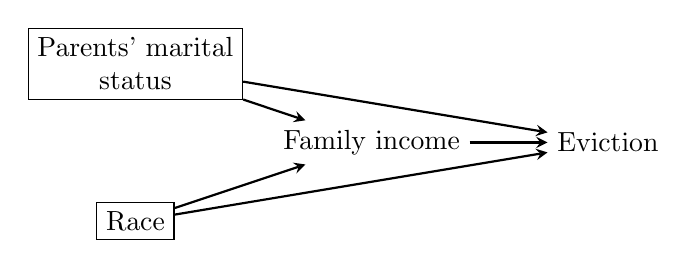
\begin{tikzpicture}[x = 1cm]
  \node (D) at (0,0) {Family income};
  \node (Y) at (3, 0) {Eviction};
  \node[draw] (X1) at  (-3,-1) {Race};
  \node[align=center,draw] (X2) at  (-3,1) {Parents' marital\\status};
  \draw[->, >=stealth, thick] (X1) -- (D);
  \draw[->, >=stealth, thick] (X1) -- (Y);
  \draw[->, >=stealth, thick] (X2) -- (D);
  \draw[->, >=stealth, thick] (X2) -- (Y);
  \draw[->, >=stealth, thick] (D) -- (Y);
  \end{tikzpicture}
\end{center}
\pause
These are identification assumptions. We are also making estimation assumptions. \\
Often the quantity of interest is causal, but be careful to \green{acknowledge the strong assumptions} required!
\end{frame}


\begin{frame}[fragile]{3. Calculate the MLE for our quantity of interest $\tau = h(\theta)$}
The true probability of eviction for a child with covariates $\vec{x}$ in a given year is
$$\tau = \pi_\text{Twice} - \pi_\text{Half}$$ \pause
\begin{enumerate}
\item Plug in the MLE estimates $\hat\beta$
\item Calculate $\hat\pi_\text{Twice}$ and $\hat\pi_\text{Half}$
\item Calculate $\hat\tau$
\end{enumerate} \vskip .3cm
All works by the \pause \blue{invariance property}.
\end{frame}

\begin{frame}[fragile]{3. Calculate the MLE for our quantity of interest $\tau = h(\theta)$}
\bblue{In code:}
\begin{footnotesize}
\begin{semiverbatim}
> colnames(X)
[1] "(Intercept)"  "married"      "raceBlack"    
     "raceHispanic" "raceOther"    "income"
\end{semiverbatim} \pause
\begin{semiverbatim}
setX <- rbind(deep_poverty = c(1, 1, 0, 0, 0, .5),
              twice_poverty = c(1, 1, 0, 0, 0, 2))
\end{semiverbatim} \pause
\begin{semiverbatim}
get.pred.diff <- function(setX, beta) \{
\end{semiverbatim} \pause
\begin{semiverbatim}
  probs <- get.pred.prob(setX, beta)
\end{semiverbatim} \pause
\begin{semiverbatim}
  difference <- probs[2] - probs[1]
\end{semiverbatim} \pause
\begin{semiverbatim}
  return(difference)
\}
\end{semiverbatim}
\end{footnotesize}
\end{frame}

\begin{frame}{A framework for doing research}
\begin{center}\begin{tikzpicture}[x = .5\textwidth, y = .5\textheight]
\node[align=left, text width = \textwidth] at (0,0) {
\begin{enumerate}
\item Define a quantity of interest $\tau$
\item Specify a model and maximize the likelihood to estimate $\hat\theta$
\item Calculate the MLE for your quantity of interest: $\hat\tau = h(\hat\theta)$
\item Simulate estimation uncertainty. Do the following thousands of times:
\begin{enumerate}
\item Draw $\tilde\theta$ from its theoretical sampling distribution
\item Calculate your quantity of interest $\tilde\tau = h\left(\tilde\theta\right)$
\end{enumerate}
\item Report your point estimate from (3) and a 95\% confidence interval from (4) in an informative graph.
\end{enumerate}
};
\node[blue] (soc) at (0.5, 0.7) {This is social science!};
\draw[->, blue, thick] (soc) to[bend left = 20] (0.07, 0.45);
\node[olive, align = center] (auto) at (-.8,0.7) {This should\\feel automatic};
\draw[->, olive, thick] (auto) to[bend right = 50] (-1, 0.2);
\draw[->, olive, thick] (auto) to[bend right = 50] (-1, 0.1);
\node[purple] (comm) at (0,-.7) {Communication matters!};
\draw[->, purple, thick] (0.4,-.7) to[bend right = 80] (0.4, -.5);
\end{tikzpicture}\end{center}
\end{frame}

\begin{frame}[fragile]{4. Simulate estimation uncertainty}
$$\tilde\beta \sim \text{Normal}\left(\hat\beta,\hat\V(\hat\beta)\right)$$
$$\tilde\pi = h(x,\tilde\beta)$$
$$\tilde\tau = \tilde\pi_\text{Twice} - \tilde\pi_\text{Half}$$
Take one draw of $\tilde{\tau}$. \pause
\begin{footnotesize}\begin{semiverbatim}
draw.sim.diff <- function(setX, beta_hat, vcov_beta_hat) \{
  beta_tilde <- t(rmvnorm(n = 1,
                          mean = beta_hat,
                          sigma = vcov_beta_hat))
  difference_tilde <- get.pred.diff(setX = setX, beta = beta_tilde)
  return(difference_tilde)
\}
\end{semiverbatim}\end{footnotesize}
\end{frame}

\begin{frame}[fragile]{4. Simulate estimation uncertainty}
Take many draws of $\tilde{\tau}$.
\begin{footnotesize}\begin{semiverbatim}
beta_hat <- opt$par
vcov_beta_hat <- -solve(opt$hessian)
set.seed(08544)
draws <- replicate(20000,
                   draw.sim.diff(setX = setX, beta_hat = beta_hat,
                                 vcov_beta_hat = vcov_beta_hat))
\end{semiverbatim}\end{footnotesize}
\end{frame}

\begin{frame}{A framework for doing research}
\begin{center}\begin{tikzpicture}[x = .5\textwidth, y = .5\textheight]
\node[align=left, text width = \textwidth] at (0,0) {
\begin{enumerate}
\item Define a quantity of interest $\tau$
\item Specify a model and maximize the likelihood to estimate $\hat\theta$
\item Calculate the MLE for your quantity of interest: $\hat\tau = h(\hat\theta)$
\item Simulate estimation uncertainty. Do the following thousands of times:
\begin{enumerate}
\item Draw $\tilde\theta$ from its theoretical sampling distribution
\item Calculate your quantity of interest $\tilde\tau = h\left(\tilde\theta\right)$
\end{enumerate}
\item Report your point estimate from (3) and a 95\% confidence interval from (4) in an informative graph.
\end{enumerate}
};
\node[blue] (soc) at (0.5, 0.7) {This is social science!};
\draw[->, blue, thick] (soc) to[bend left = 20] (0.07, 0.45);
\node[olive, align = center] (auto) at (-.8,0.7) {This should\\feel automatic};
\draw[->, olive, thick] (auto) to[bend right = 50] (-1, 0.2);
\draw[->, olive, thick] (auto) to[bend right = 50] (-1, 0.1);
\node[purple] (comm) at (0,-.7) {Communication matters!};
\draw[->, purple, thick] (0.4,-.7) to[bend right = 80] (0.4, -.5);
\end{tikzpicture}\end{center}
\end{frame}

\begin{frame}{5. Report results}
We recommend reporting
\begin{itemize}
\item your point estimate $\hat\tau$ \onslide<2->{(the MLE by the invariance property)}
\item a 95\% quantile-based confidence interval
\end{itemize}
\onslide<3->{
\begin{center}
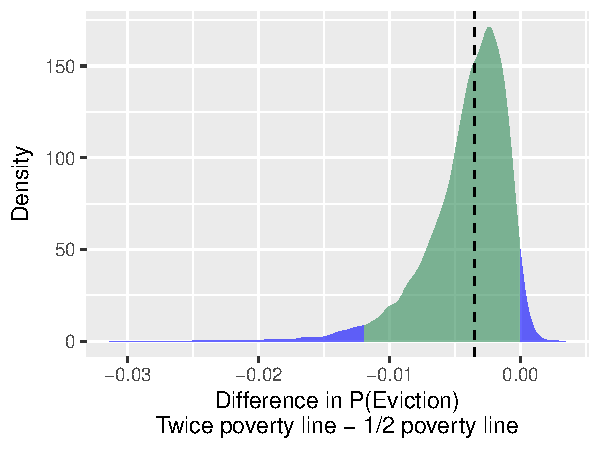
\includegraphics[width=.6\textwidth]{figs/pred_diff}
\end{center}
}
\end{frame}

\begin{frame}{A framework for doing research}
\begin{center}\begin{tikzpicture}[x = .5\textwidth, y = .5\textheight]
\node[align=left, text width = \textwidth] at (0,0) {
\begin{enumerate}
\item Define a quantity of interest $\tau$
\item Specify a model and maximize the likelihood to estimate $\hat\theta$
\item Calculate the MLE for your quantity of interest: $\hat\tau = h(\hat\theta)$
\item Simulate estimation uncertainty. Do the following thousands of times:
\begin{enumerate}
\item Draw $\tilde\theta$ from its theoretical sampling distribution
\item Calculate your quantity of interest $\tilde\tau = h\left(\tilde\theta\right)$
\end{enumerate}
\item Report your point estimate from (3) and a 95\% confidence interval from (4) in an informative graph.
\end{enumerate}
};
\node[blue] (soc) at (0.5, 0.7) {This is social science!};
\draw[->, blue, thick] (soc) to[bend left = 20] (0.07, 0.45);
\node[olive, align = center] (auto) at (-.8,0.7) {This should\\feel automatic};
\draw[->, olive, thick] (auto) to[bend right = 50] (-1, 0.2);
\draw[->, olive, thick] (auto) to[bend right = 50] (-1, 0.1);
\node[purple] (comm) at (0,-.7) {Communication matters!};
\draw[->, purple, thick] (0.4,-.7) to[bend right = 80] (0.4, -.5);
\end{tikzpicture}\end{center}
\end{frame}


\section[2]{Practice 2}

\begin{frame}
\Huge\centering \blue{More practice.}
\end{frame}

\begin{frame}
\frametitle{Different quantity of interest}
\pause
What is the probability of any eviction from birth to age 9, for a randomly sampled child born in a large American city? \\
\pause
$$\begin{aligned}
\pi^\text{Ever}_i = \P(\text{Ever evicted}\mid \vec{X}_i) \pause &= 1 - \P(\text{Never evicted}\mid \vec{X}_i) \\ \pause
&= 1- \prod_{t=1}^9 (1 - \P(\text{Evicted at age }t\mid \vec{X}_i)) \\ \pause
&= 1 - (1 - \pi_i)^9
\end{aligned}$$
\bigskip
The model is the same. We just changed the \blue{quantity of interest}. \footnote{Note: We assume independence between eviction in each year, and a constant risk over time. This corresponds to an Exponential survival model.\vskip .2cm}
\end{frame}


\begin{frame}[fragile]{Calculate the MLE for our quantity of interest $\tau = h(\theta)$}
The true probability of eviction for a child with covariates $\vec{x}$ in a given year is
$$\pi_i = 1 - \exp(-\exp(\vec{X}_i\vec\beta))$$ \pause
The true probability of ever being evicted is:
$$\pi^\text{Ever}_i = h\left(\vec{x},\vec\beta\right) \pause = 1 - (1 - \pi_i)^9$$ \pause
We might want to report the \blue{weighted sample average} of the $\pi_i$.
$$\bar\pi^\text{Ever} = \frac{1}{\sum w_i} \sum_{i=1}^n w_i \pi^\text{Ever}_i$$
Plug in the MLE estimates $\hat\beta$ and solve! \pause \blue{(invariance property)}. \vskip .2cm \pause
\begin{footnotesize}\blue{Why weight?} Assuming the model is correctly specified, this is representative of the probability of eviction by age 9 for a randomly sampled child born in a U.S. city with population over 200,000 in 1998-2000.\end{footnotesize}
\end{frame}

\begin{frame}[fragile]{Calculate the MLE for our quantity of interest $\tau = h(\theta)$}
\bblue{In code:}
\begin{footnotesize}
\begin{semiverbatim}
get.pred.cum <- function(setX, beta, weights) \{
  ## Calculate the linear predictor
  eta <- setX \%*\% beta
  ## Transform by the inverse link function
  prob_annual <- 1 - exp(-exp(eta))
  prob_cum <- 1 - (1 - prob_annual) ^ 9
  return(weighted.mean(prob_cum,
                       w = weights))
  return(prob_cum)
\}
\end{semiverbatim}
\end{footnotesize}
\end{frame}

\begin{frame}{A framework for doing research}
\begin{center}\begin{tikzpicture}[x = .5\textwidth, y = .5\textheight]
\node[align=left, text width = \textwidth] at (0,0) {
\begin{enumerate}
\item Define a quantity of interest $\tau$
\item Specify a model and maximize the likelihood to estimate $\hat\theta$
\item Calculate the MLE for your quantity of interest: $\hat\tau = h(\hat\theta)$
\item Simulate estimation uncertainty. Do the following thousands of times:
\begin{enumerate}
\item Draw $\tilde\theta$ from its theoretical sampling distribution
\item Calculate your quantity of interest $\tilde\tau = h\left(\tilde\theta\right)$
\end{enumerate}
\item Report your point estimate from (3) and a 95\% confidence interval from (4) in an informative graph.
\end{enumerate}
};
\node[blue] (soc) at (0.5, 0.7) {This is social science!};
\draw[->, blue, thick] (soc) to[bend left = 20] (0.07, 0.45);
\node[olive, align = center] (auto) at (-.8,0.7) {This should\\feel automatic};
\draw[->, olive, thick] (auto) to[bend right = 50] (-1, 0.2);
\draw[->, olive, thick] (auto) to[bend right = 50] (-1, 0.1);
\node[purple] (comm) at (0,-.7) {Communication matters!};
\draw[->, purple, thick] (0.4,-.7) to[bend right = 80] (0.4, -.5);
\end{tikzpicture}\end{center}
\end{frame}

\begin{frame}[fragile]{4. Simulate estimation uncertainty}
$$\tilde\beta \sim \text{Normal}\left(\hat\beta,\hat\V(\hat\beta)\right)$$
$$\tilde\pi = h(x,\tilde\beta)$$
$$\tilde\pi^\text{Ever}_i = h\left(\vec{x},\tilde\beta\right) \pause = 1 - (1 - \tilde\pi_i)^9$$ \pause
$$\tilde{\bar\pi}^\text{Ever} = \frac{1}{\sum w_i} \sum_{i=1}^n w_i \tilde\pi^\text{Ever}_i$$ \pause
Take one draw of $\tilde{\bar\pi}^\text{Ever}$. \pause
\begin{footnotesize}\begin{semiverbatim}
draw.sim.cum <- function(setX, beta_hat, vcov_beta_hat, weights) \{
  beta_tilde <- t(rmvnorm(n = 1,
                          mean = beta_hat,
                          sigma = vcov_beta_hat))
  cum_tilde <- get.pred.cum(setX = setX, beta = beta_tilde, weights = weights)
  return(cum_tilde)
\}
\end{semiverbatim}\end{footnotesize}
\end{frame}

\begin{frame}[fragile]{4. Simulate estimation uncertainty}
Take many draws of $\tilde{\bar\pi}^\text{Ever}$.
\begin{footnotesize}\begin{semiverbatim}
beta\_hat <- opt$par
vcov\_beta\_hat <- -solve(opt$hessian)
set.seed(08544)
draw.sim.cum(setX = X, beta\_hat = opt$par,
             vcov\_beta\_hat = -solve(opt$hessian),
             weights = d$m1natwt)
\end{semiverbatim}\end{footnotesize}
\end{frame}

\begin{frame}{A framework for doing research}
\begin{center}\begin{tikzpicture}[x = .5\textwidth, y = .5\textheight]
\node[align=left, text width = \textwidth] at (0,0) {
\begin{enumerate}
\item Define a quantity of interest $\tau$
\item Specify a model and maximize the likelihood to estimate $\hat\theta$
\item Calculate the MLE for your quantity of interest: $\hat\tau = h(\hat\theta)$
\item Simulate estimation uncertainty. Do the following thousands of times:
\begin{enumerate}
\item Draw $\tilde\theta$ from its theoretical sampling distribution
\item Calculate your quantity of interest $\tilde\tau = h\left(\tilde\theta\right)$
\end{enumerate}
\item Report your point estimate from (3) and a 95\% confidence interval from (4) in an informative graph.
\end{enumerate}
};
\node[blue] (soc) at (0.5, 0.7) {This is social science!};
\draw[->, blue, thick] (soc) to[bend left = 20] (0.07, 0.45);
\node[olive, align = center] (auto) at (-.8,0.7) {This should\\feel automatic};
\draw[->, olive, thick] (auto) to[bend right = 50] (-1, 0.2);
\draw[->, olive, thick] (auto) to[bend right = 50] (-1, 0.1);
\node[purple] (comm) at (0,-.7) {Communication matters!};
\draw[->, purple, thick] (0.4,-.7) to[bend right = 80] (0.4, -.5);
\end{tikzpicture}\end{center}
\end{frame}

\begin{frame}{5. Report results}
We recommend reporting
\begin{itemize}
\item your point estimate $\hat\tau$ \onslide<2->{(the MLE by the invariance property)}
\item a 95\% quantile-based confidence interval
\end{itemize}
\onslide<3->{
\begin{center}
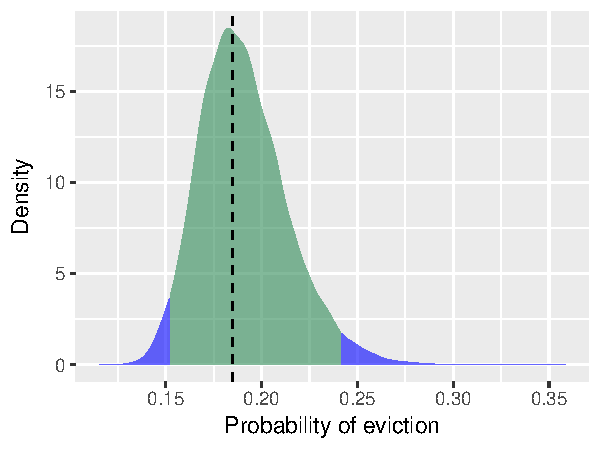
\includegraphics[width=.6\textwidth]{figs/pred_cum}
\end{center}
}
\end{frame}

\begin{frame}{A framework for doing research}
\begin{center}\begin{tikzpicture}[x = .5\textwidth, y = .5\textheight]
\node[align=left, text width = \textwidth] at (0,0) {
\begin{enumerate}
\item Define a quantity of interest $\tau$
\item Specify a model and maximize the likelihood to estimate $\hat\theta$
\item Calculate the MLE for your quantity of interest: $\hat\tau = h(\hat\theta)$
\item Simulate estimation uncertainty. Do the following thousands of times:
\begin{enumerate}
\item Draw $\tilde\theta$ from its theoretical sampling distribution
\item Calculate your quantity of interest $\tilde\tau = h\left(\tilde\theta\right)$
\end{enumerate}
\item Report your point estimate from (3) and a 95\% confidence interval from (4) in an informative graph.
\end{enumerate}
};
\node[blue] (soc) at (0.5, 0.7) {This is social science!};
\draw[->, blue, thick] (soc) to[bend left = 20] (0.07, 0.45);
\node[olive, align = center] (auto) at (-.8,0.7) {This should\\feel automatic};
\draw[->, olive, thick] (auto) to[bend right = 50] (-1, 0.2);
\draw[->, olive, thick] (auto) to[bend right = 50] (-1, 0.1);
\node[purple] (comm) at (0,-.7) {Communication matters!};
\draw[->, purple, thick] (0.4,-.7) to[bend right = 80] (0.4, -.5);
\end{tikzpicture}\end{center}
\end{frame}


\begin{frame}

\begin{huge}Appendix: Hypothesis tests\end{huge} \vskip .5cm
We went through this quickly. Please ask questions on Piazza or in office hours and we will try to clarify! These last two slides have what we wrote on the board.

\end{frame}

\begin{frame}{Hypothesis test for a mean}
This should be review from the fall.
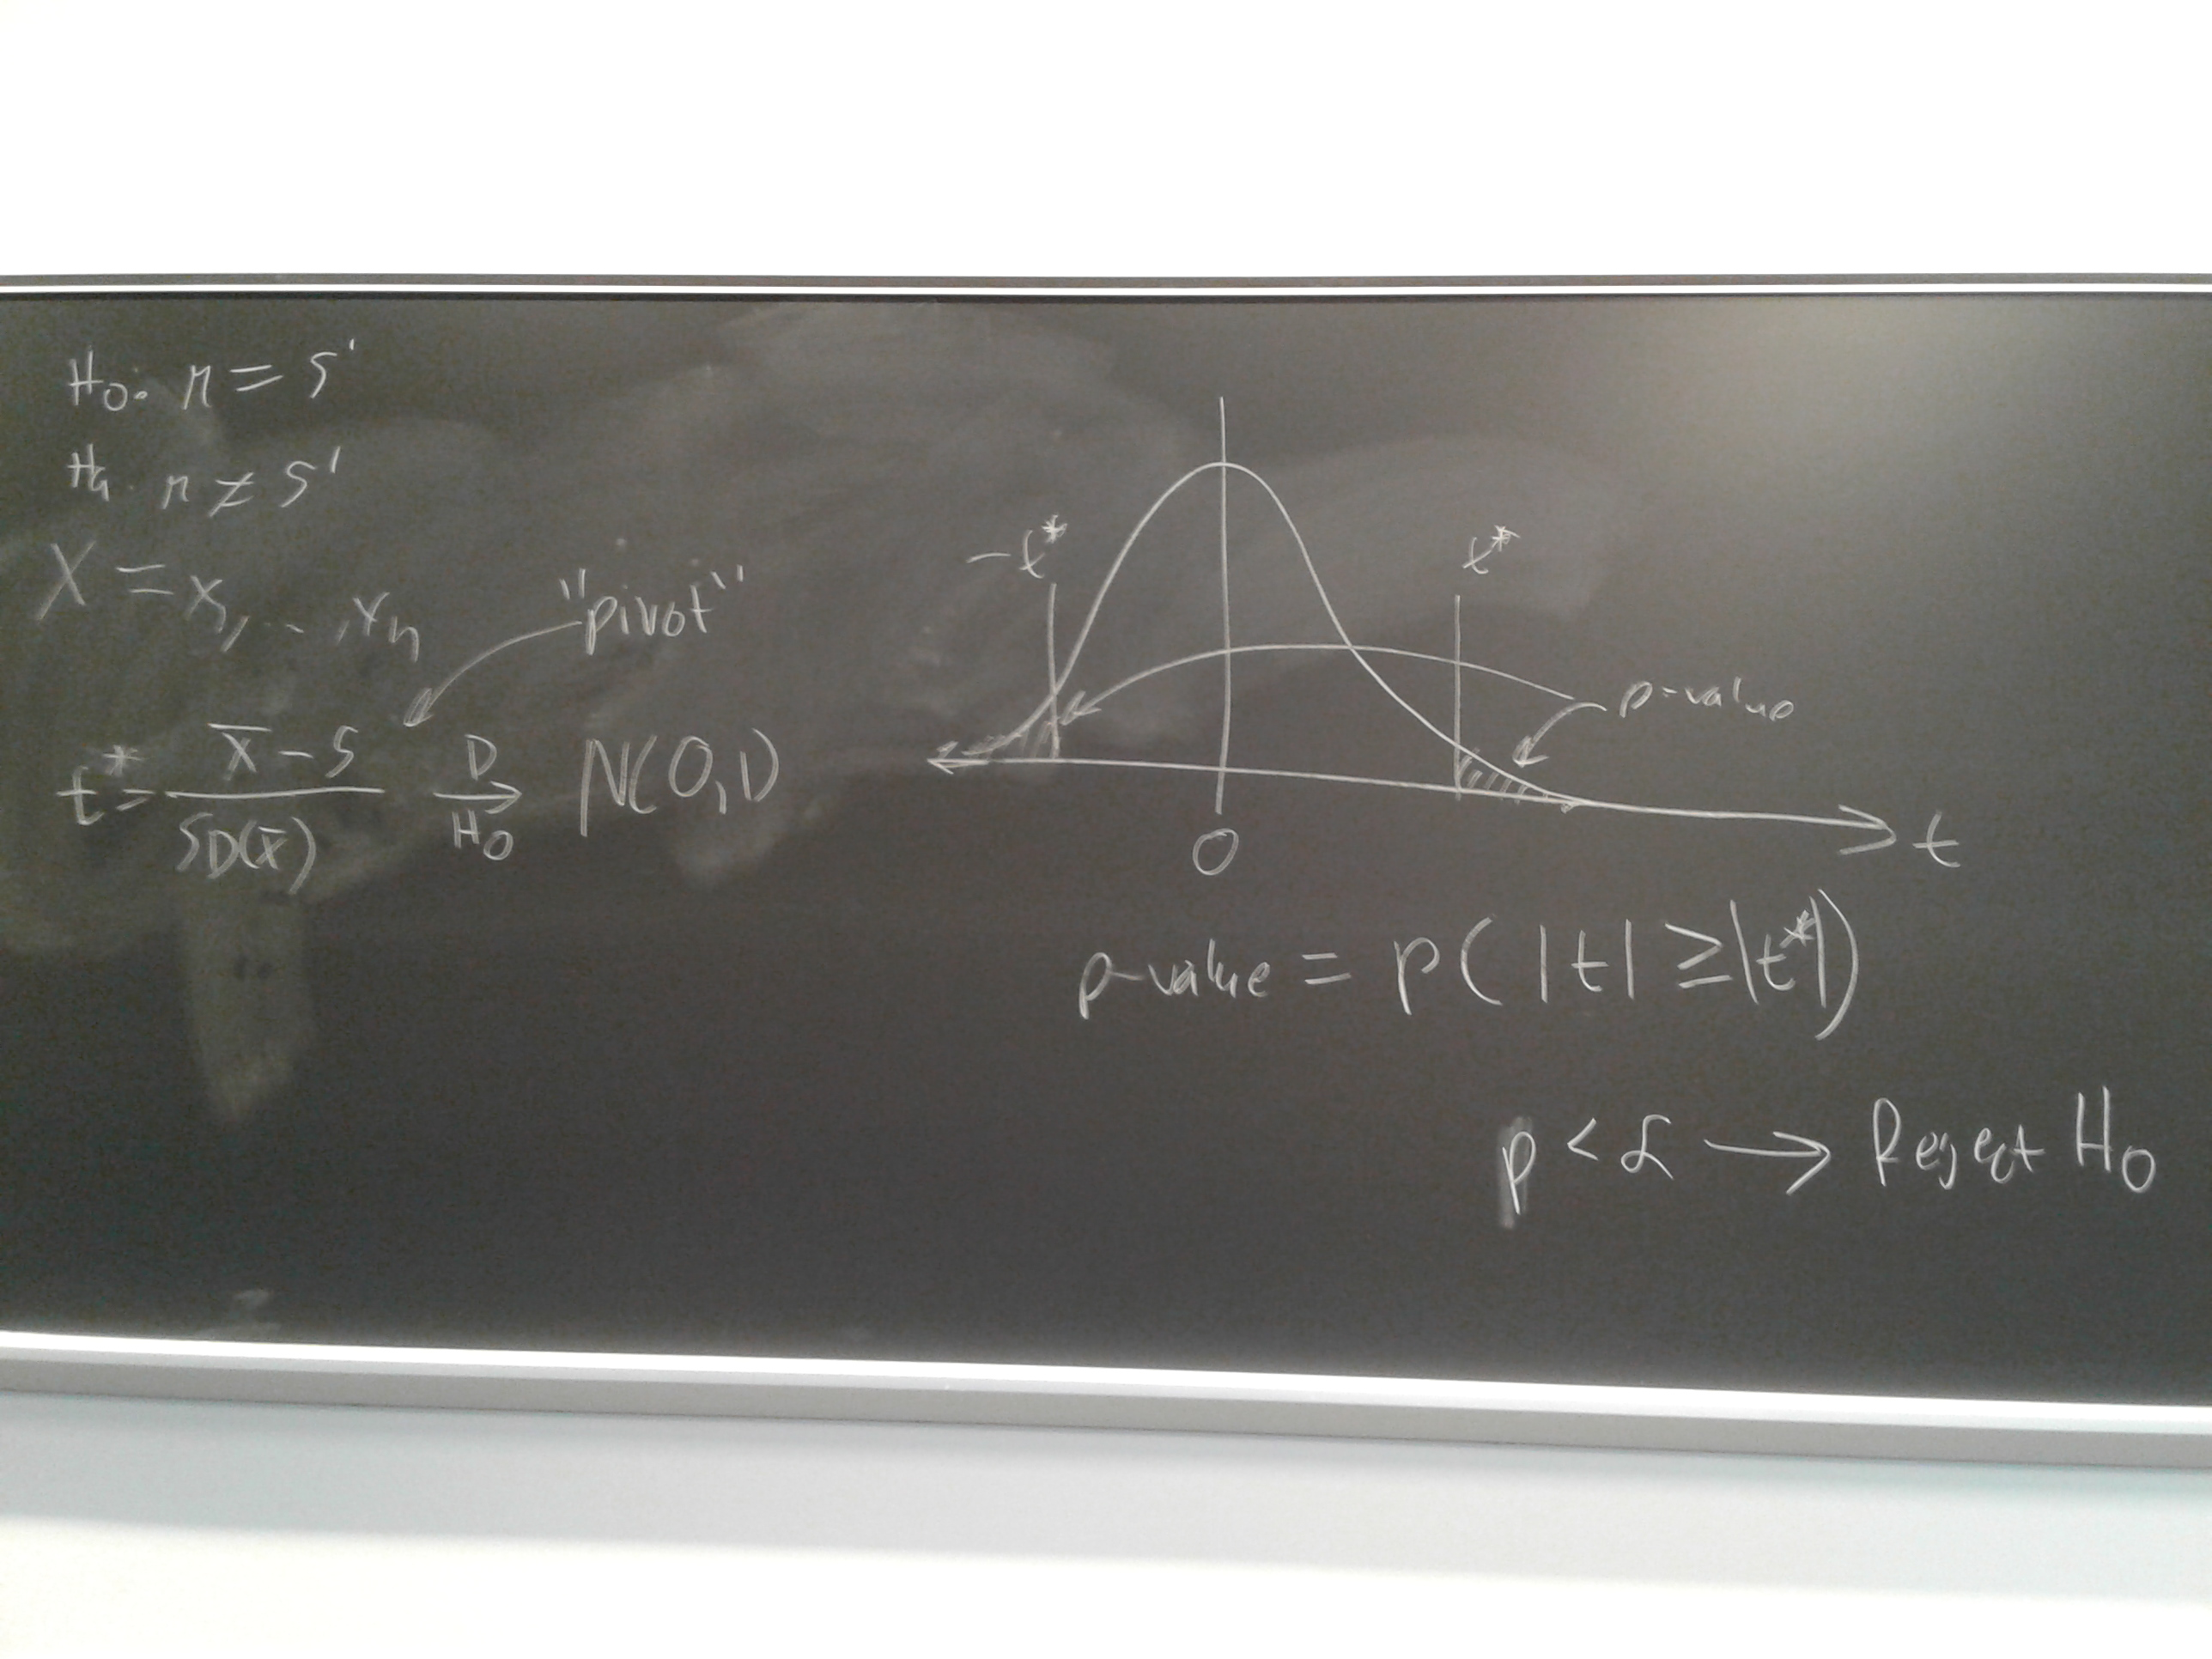
\includegraphics[width = \textwidth]{figs/TTest}
\end{frame}

\begin{frame}{Likelihood ratio test}
This is new this semester.
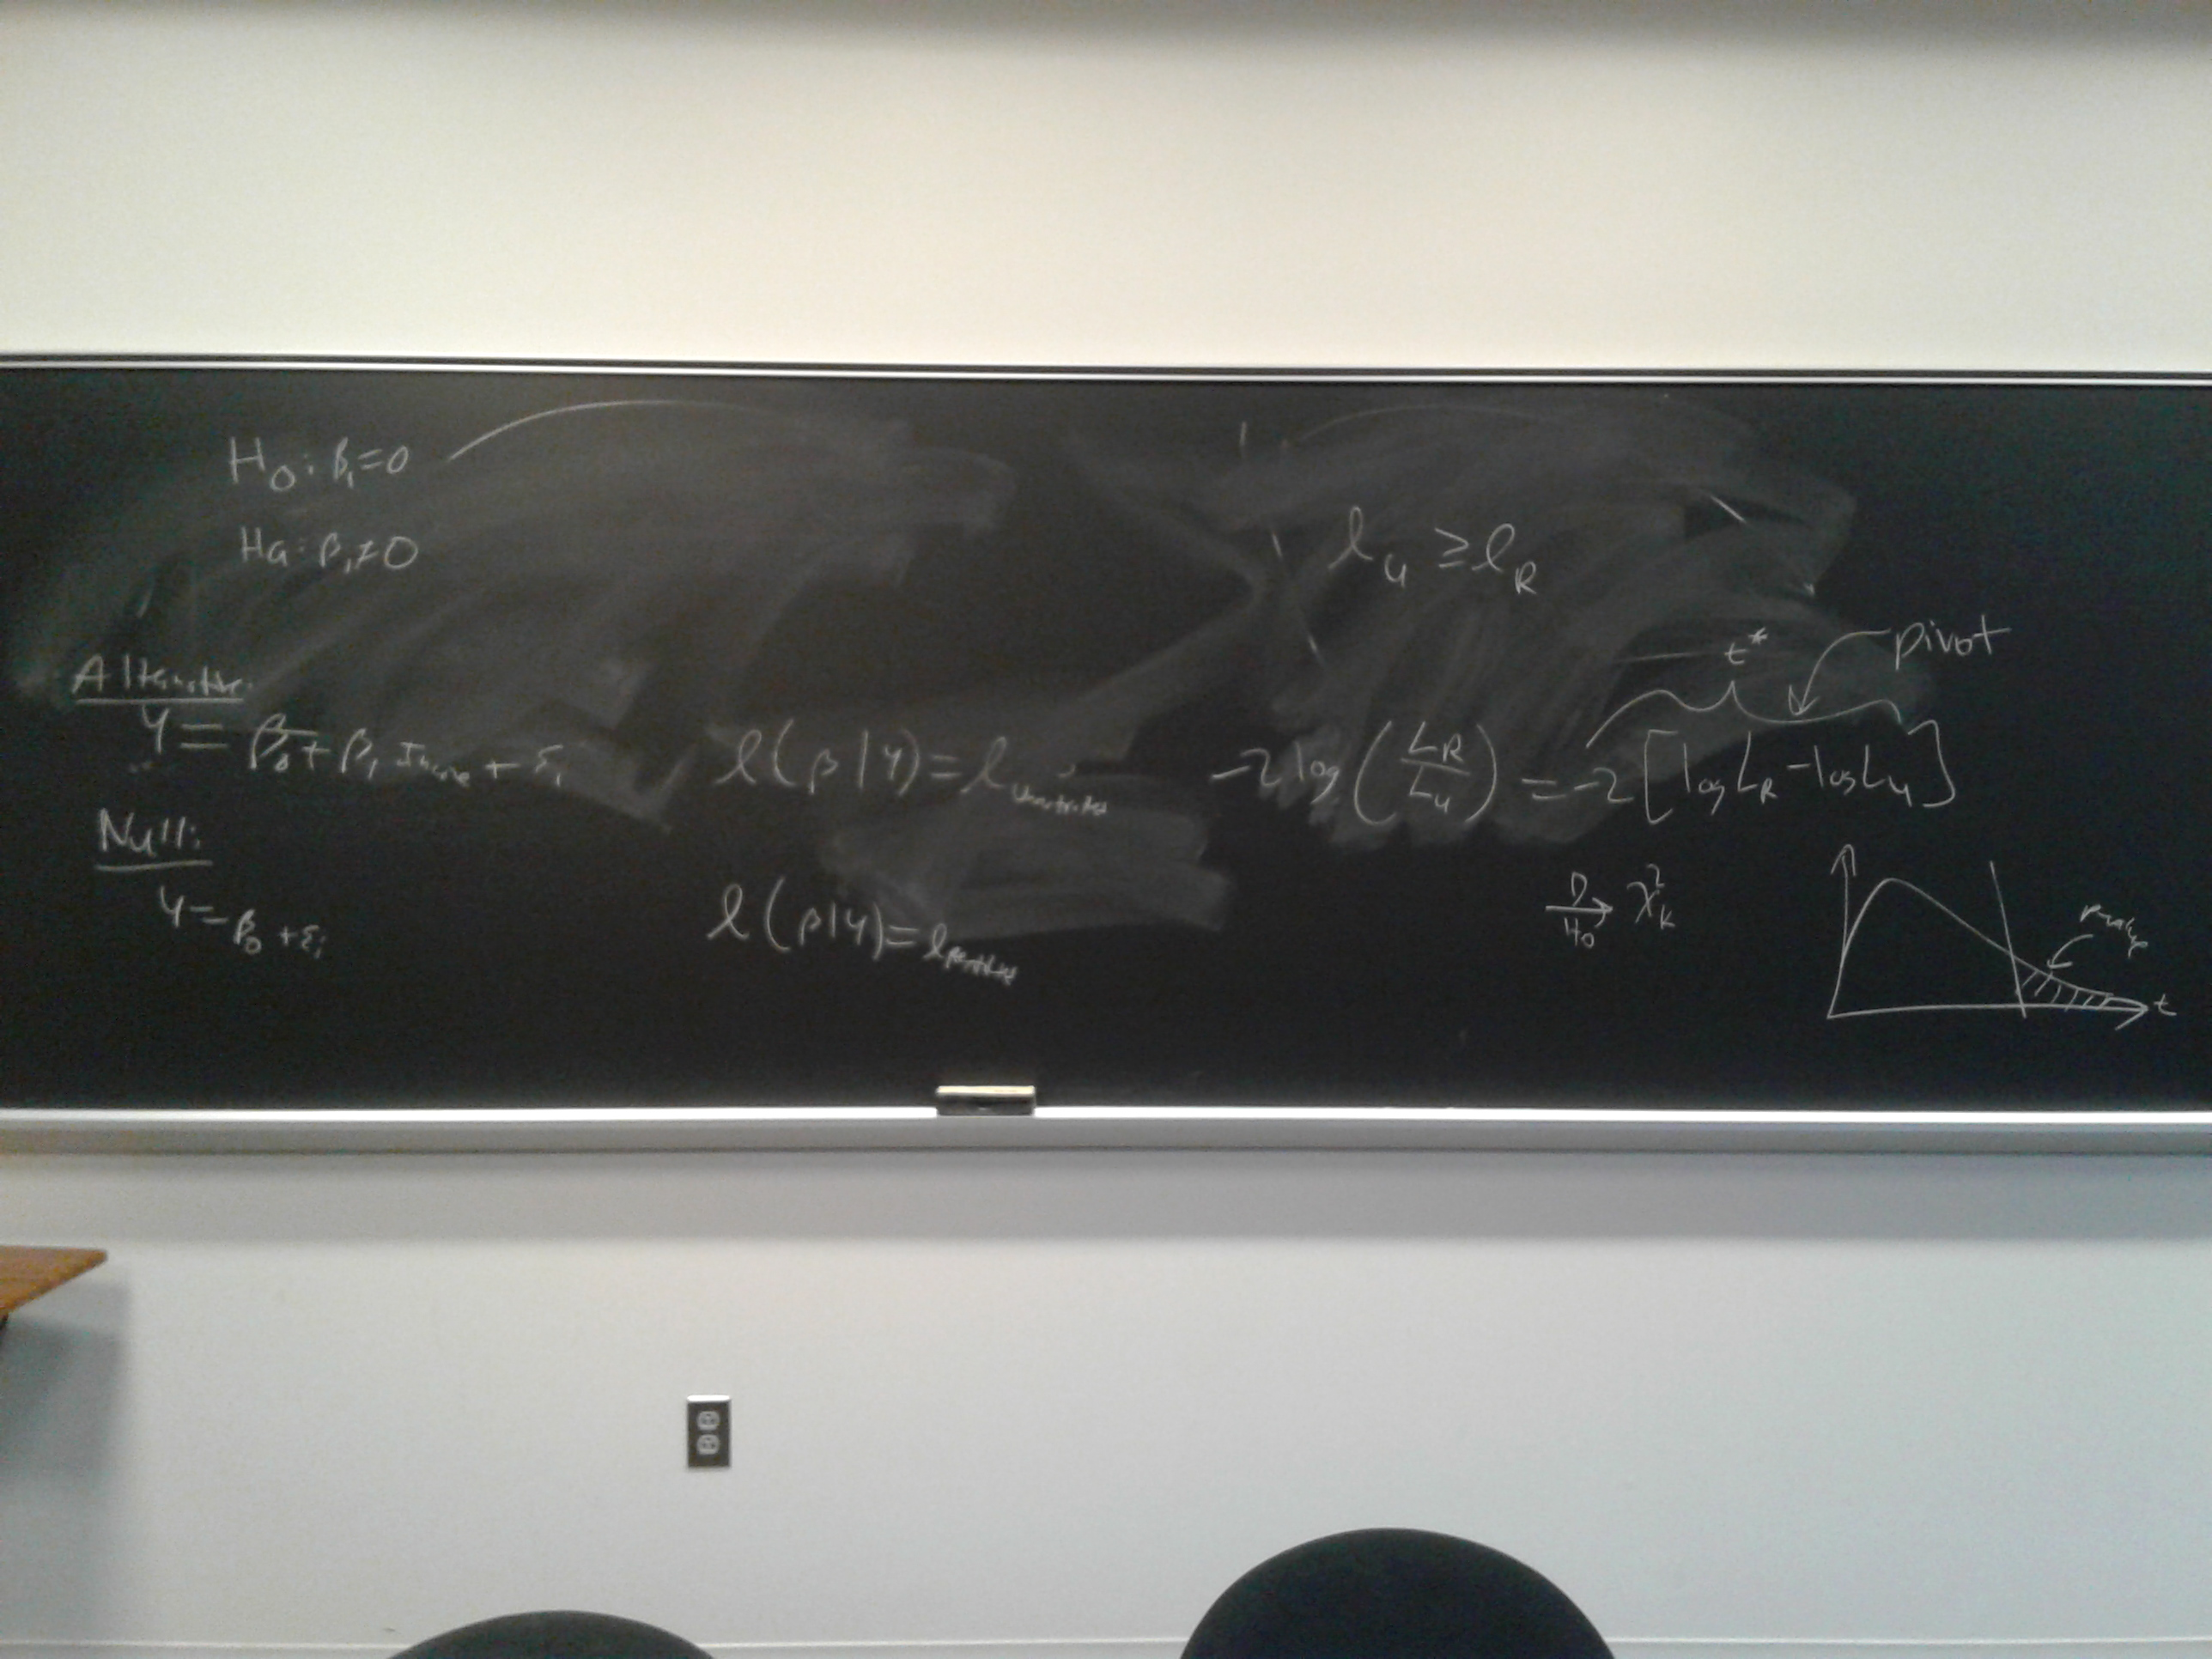
\includegraphics[width = \textwidth]{figs/LRTest}
\end{frame}


\end{document}
